\documentclass[10pt,onecolumn]{paper}

\usepackage{fancybox}
\usepackage{times}

\usepackage[draft, marginclue, footnote]{fixme}
% with draft mode, all fixes are displyed
% with non-draft, non fatal fixmes are not displayed and fatal ones
% produce errors in compilation

\usepackage[utf8]{inputenc}

\usepackage{graphicx}
\usepackage{url}
\usepackage{subcaption}
\usepackage{mdwlist}
\usepackage{paralist}
\usepackage{xspace}
\usepackage{multirow}
\usepackage[procnames]{listings}
\usepackage{rotating}
\usepackage{wrapfig}
\usepackage{cite}
\usepackage{algorithmic}
\usepackage{textcomp}
\usepackage{booktabs}
\usepackage{amsmath}
\usepackage{verbatim}
\usepackage{cleveref}
\usepackage{todonotes}
\usepackage{tcolorbox}
\usepackage{placeins}

\newtcolorbox{mybox}[1]{colback=red!5!white,colframe=red!75!black,fonttitle=\bfseries,title=#1}
\input{defs}

\newcommand{\HRule}{\rule{\linewidth}{0.5mm}}
\begin{document}

\begin{titlepage}
\begin{center}

% Title
\HRule \\[0.4cm]
{ \huge \bfseries Report on the testbed results of the BattleMesh V10 \\[0.4cm] }

\HRule \\[1.5cm]

\begin{minipage}{0.4\textwidth}
\begin{flushleft} \large
Bastian \textsc{Bittorf}\\
Alessandro \textsc{Gnagni}\\
Leonardo \textsc{Maccari}\\
Gioacchino \textsc{Mazzucco}\\
Claudio \textsc{Pisa}\\
Jehan \textsc{Tremback} \\
\end{flushleft}
\end{minipage}
\begin{minipage}{0.4\textwidth}
\end{minipage}

\vfill
{\large Abstract}
\HRule \\[0.4cm]
\begin{flushleft}
\emph{The Wireless Battle of the Mesh is an yearly event that brings together
people from across the world to test and compare the performance of different routing
protocols for ad-hoc and mesh networks, like Babel, B.A.T.M.A.N., BMX6, OLSR,
802.11s. Every year the community gathers and set-up a testbed on which the
protocols are run, developed, debugged and tested, and some performance
measures are extracted. While the initial spirit of the event was to set-up a
competition between the protocols (as the name suggests), with time it changed
into a moment of exchange of experience, collective development of
innovations in the field of mesh networks and wireless open source
networking software. This document reports on the experimental results of the tenth edition
of the Battle of The Mesh event.}
\end{flushleft}
\vskip2cm

\vfill

% Bottom of the page
{\large \today}

\end{center}
\end{titlepage}


\section{BattleMesh v10}
The Battle of the Mesh (WBM), as the official website says:
\begin{quote}
It is a tournament with a social character. If you are a mesh networking
enthusiast, community networking activist, or have an interest in mesh networks
you might want to check this out!

The goal of the WirelessBattleMesh events is to set-up hands-on testbed for each
available mesh routing protocol with a standard test procedure for the different
mesh networks. During the different WBM events, similar hardware and software
configuration will be used based on the OpenWRT BoardSupportPackage and packages
for each protocol implementation. The WBM events are also a great opportunity to
develop testing tools for PHY/MAC radio layers (drivers, scripts and PHY
analyzers).
\end{quote}

WBM is now at its tenth edition, and is organized by a motivated and large group
of people (approximately 80-100 participants in the whole week in the last
editions from 2-3 continents). 

\section{The Testbed}
This year, the testbed was realized with 17 TP-Link WDR4300 routers, equipped
with two wireless interfaces (operating in the 2.4 and 5.0 GHz bands), and 5
Ubiquiti Unifi AC Pro. The latter were used to perform local testing and support
to the tests, but did not participate to the routing, since they are equipped
with a different chipset. The nodes were configured to set-up two independent
networks, a ``management'' network, running on the 2.4GHz, and a ``testing''
network, running on the 5 GHz. The management network was configured with the
IEEE 802.11s protocol, and was used only to access the nodes and perform
tasks. The testing network was made with interfaces configured in ad-hoc mode
and, for each test, was using a specific routing protocol. 

\Cref{fig:topo} reports the topology of the network as exported by one of the
network node, when running the OLSRv1 protocol. This topology was used to
understand and roughly guess the property of the network. The underlying image
is the map of \textit{Volkskundemuseum Wien}\footnote{The Austrian Museum of
Folk Life And Folk Art, Laudongasse 15-19, Vienna, Austria}
that hosted the event, roughly, the distance from node 9 to node 17 is about
75m, and the width of the main room is about 8m (the main room is the room where
nodes 1,4,7,6,31 are placed and where the conference took place).


Routers numbered from 1 to 17 are the TP-Link, while router 31 is an Ubiquiti
router that is used in this case to extract the network topology. In the real
tests this router does not participate to the network functioning. The
transparency of the links represents the badness of the link quality as reported
by the OLSRv1 protocol, using the ETX metric. A solid link means ETX =
1 (good link), while a transparent link means ETX $>$ 1 (the highest, the worse).


\begin{figure}[!htb]
  \centering
  \includegraphics[width=\linewidth]{images/map.png}
  \caption{Network topology, as exported from the OLSRv1 protocol} 
  \label{fig:topo}
\end{figure}%

Note that the topology in \cref{fig:topo} does not necessarily represent the
topology used by other routing protocols, but gives an approximate idea of what
links are directly connected. Based on this topology, exported in the netJSON
format\footnote{A generic format for exporting a network topology, see
\url{http://netjson.org}}, we calculated the weighted shortest path between any couple of node,
using the networkX python graph
library. We repeated the process twice, with two different transmission power
level for the testing network. With the transmission power set to 17dBm the
network was considered too dense, and thus of little interest for the routing
function. Therefore the power was lowered to 10dBm, and produced the
distribution of path costs reported in \cref{fig:ETXrank}. Each entry is computed
as follows, given the network graph and a couple of nodes (A, B), the shortest
path between A and B is computed via networkX and then the sum of the ETX values
for the path is done\footnote{For the code used for this task, see
\url{https://github.com/battlemesh/battlemeshv10-testbed/blob/master/tests/failure_recovery/parser_scripts/parse_json.py}}. We selected four nodes
to perform the tests, node 8, 9, 17, and 2, that are at the extreme ends of the
topology. \cref{fig:ETXrank} reports the corresponding shortest path costs in
the ranking.

\begin{figure}[!htb]
  \centering
  \includegraphics[width=\linewidth]{images/route_lenght_distribution.png}
  \caption{The ranked list of the ETX weight of all the shortest paths in the
    network.} 
  \label{fig:ETXrank}
\end{figure}

\subsection{The Protocols and the Experiments}

Several protocols were tested during the WBM, not all the protocols (or their
variants) have been tested on all the configuration. \Cref{tab:protocols}
reports the list of the protocols, a brief description, and the link to the
source code. 

\begin{table}
    \centering
    \begin{tabular}{ll}
        \emph{Name} & \emph{Desciption} \\
        \midrule
        BABEL & Distance-vector LIII routing protocol \\
        BATMAN Advanced v4 & Source Routed LII routing protocol \\
        BATMAN Advanced v5 & Source Routed LII routing protocol (experimental)\\
        BMX7  & Source Routed LIII routing protocol \\
        BMX7TUN   & BMX7 with IP tunnel support\\
        OLSRv1 &  Link state LIII routing protocol\\
        OLSRv2 &  Link state LIII routing protocol\\
        OLSRv2\_MPR  & OLSRv2 with MPR enabled\\
        \bottomrule
    \end{tabular}
    \caption{The list of tested protocols}
    \label{tab:protocols}
\end{table}

Four out of six days that make the WBM were devoted to set-up the testbed, and
only the last two were dedicated to the testing itself. The procedure of set-up
and testing is error prone due to a vast set of reasons that range from the need
to use a recent OpenWRT/LEDE version, the potential incompatibility with the
last version of the protocols, their configuration, and last, but not least, the
eventual bugs that are found while testing and need to be fixed. This is a very
important part of the WBM, possibly the most important under the technical
point of view (the social side of the WBM as equally important). During the
tests the developers of the protocols (that are generally present at the event)
test new features, compare different strategies and inevitably stumble upon
unknown bugs in their protocols. This process is vital for them to improve their
software and stabilize their code, and is arguably even more important than the
results of the tests themselves. 

Four set of experiments were planned, and three were fully performed:
\bi
\ii Ping test: a session of 100 pings from node 8 to 17, 8 to 2, 9 to 17, and 9
to 2 were performed to measure the loss and the delay distribution. This test
was repeated only once.
\ii iperf test: a batch of 10 TCP iperf sessions were run (10s each) between node 8
and 17 and from node 9 to node 2. This experiment was repeated with two more
variants, one in which node 14 and 10 were running another iperf with a 5Mbps
limit, and a second one in which 4 5Mbps session was running between other
nodes. These added sessions were not recorded but where used to increase
the level of congestion in the central part of the network.
\ii Airtime Fairness tests: in this case we repeated the iperf tests with and
without the Airtime Fairness enabled.
\ii pingall test: in this experiment, a random subset of all the possible
couples was taken and an iperf session was performed. This test should have been
repeated for all the protocols, with and without Airtime fairness enabled, but
was not possible to complete.
\ei

\section{The Results}

\subsection{Ping Tests}

\Cref{fig:pingloss} reports the percentage of lost packets in the ping tests. It
shows that OLSRv1 and BMX are the ones that choose paths that are more
conservative, so they deliver all or almost all their pings. OLSRv2, BATMAN4
and, to a lower extent BABEL are the ones that, instead, tend to choose paths
that are more lossy. BATMAN5 largely underperforms compared to the others. This
is an example of a typical situation in the WBM. BATMAN5 does not have a stable
release, and the developers brought to the WBM a testing version, to initially
study its performance. During the tests, these outlier performances made it
possible to spot the presence of previously unknown software bugs, which become
visible only when tested on networks larger than a certain size. 
It was not possible to patch BATMAN5 before the end of the WBM and thus, from
now on the results of BATMAN5 are omitted. 

\begin{figure}[!htb]
  \centering
  \includegraphics[width=.9\linewidth]{images/failure_test_loss-IPv6.png}
  \caption{The percentage of lost packets per protocol}
    \label{fig:pingloss}
\end{figure}

\Cref{fig:delaydist} reports data about the distribution of the RTT measured
with ping. What clearly emerges is that BMX is consistently using paths with
larger delays, and that BABEL on three cases over 4 has a very large range of
values. OLSRv2 performs worse than OLSRv1 in the majority of the cases, with
delays comparable to BATMAN. Note that OLSRv2, BATMAN, and BABEL are advantaged
in this comparison, since they have non-zero loss. It is reasonable to assume
that the packets that could not be delivered, if they could reach the
destination would probably have a large RTT.

\begin{figure}[!htb]
  \centering
  \includegraphics[width=.9\linewidth]{images/failure_test_delay-IPv6.png}
  \caption{The values of the 10th percentile, 90th percentile, and median value
    of the RTT for all the pings}
  \label{fig:delaydist}
\end{figure}


Finally,
\cref{fig:delaysequence1,fig:delaysequence2,fig:delaysequence3,fig:delaysequence4}
report the whole set of RTT measured for each run. Note that the tests were done
in sequence, so the network conditions may have varied from one test to the next
one, note also the log scale on y axis. It is clear that there are two
phenomenons, one is the difference from one protocol to another that impacts the
median value, the other is the presence of many outliers that influence the
whiskers of \cref{fig:delaydist}.

\begin{figure}[!htb]
  \centering
  \includegraphics[width=.9\linewidth]{images/failure_test_delay_distribution-IPv6-1-timesequence.png}
    \caption{The values of the RTT per each ping, 9 to 17}
  \label{fig:delaysequence1}
\end{figure}

\begin{figure}[!htb]
  \centering
  \includegraphics[width=.9\linewidth]{images/failure_test_delay_distribution-IPv6-2-timesequence.png}
    \caption{The values of the RTT per each ping, 9 to 2}
  \label{fig:delaysequence2}
\end{figure}

\begin{figure}[!htb]
  \centering
  \includegraphics[width=.9\linewidth]{images/failure_test_delay_distribution-IPv6-3-timesequence.png}
    \caption{The values of the RTT per each ping, 8 to 17}
  \label{fig:delaysequence3}
\end{figure}

\begin{figure}[!htb]
  \centering
  \includegraphics[width=.9\linewidth]{images/failure_test_delay_distribution-IPv6-4-timesequence.png}
    \caption{The values of the RTT per each ping, 8 to 2}
  \label{fig:delaysequence4}
\end{figure}

\begin{figure}[p]
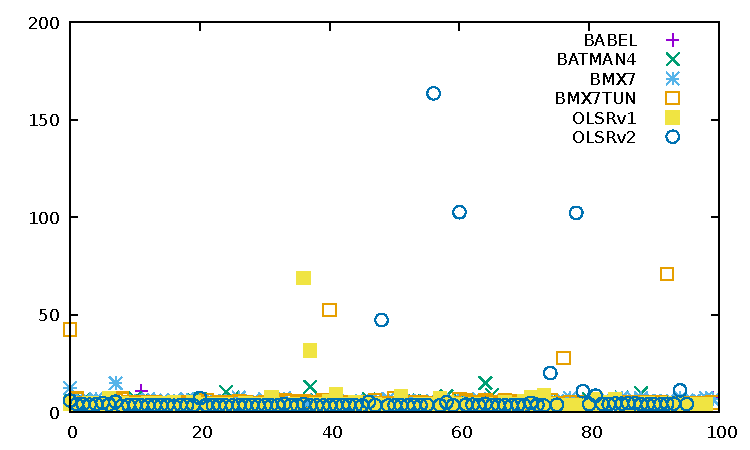
\includegraphics[width=0.48\linewidth]{images/scatter-failuretest-node8-fc00:17::1.pdf}\hfill%
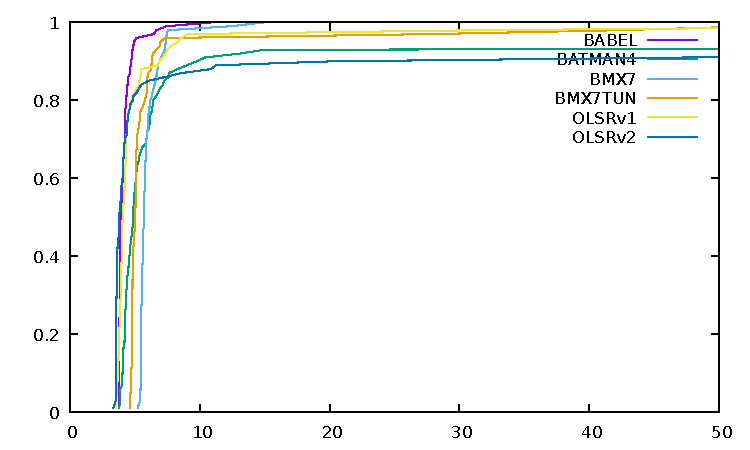
\includegraphics[width=0.48\linewidth]{images/cdf-failuretest-node8-fc00:17::1.pdf}

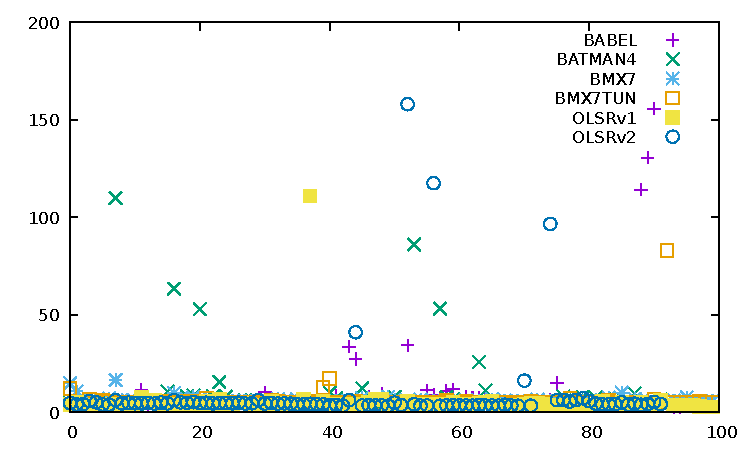
\includegraphics[width=0.48\linewidth]{images/scatter-failuretest-node8-fc00:2::1.pdf}\hfill%
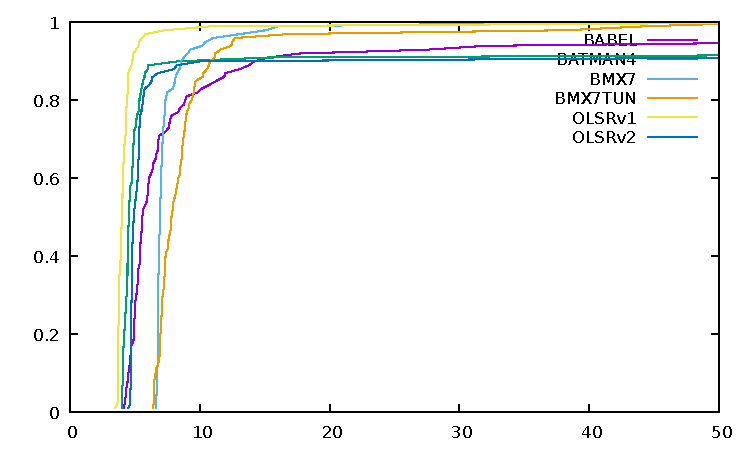
\includegraphics[width=0.48\linewidth]{images/cdf-failuretest-node9-fc00:17::1.pdf}

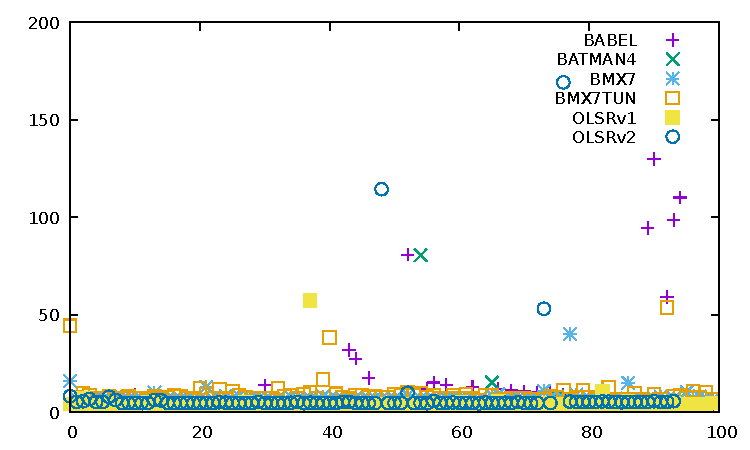
\includegraphics[width=0.48\linewidth]{images/scatter-failuretest-node9-fc00:17::1.pdf}\hfill%
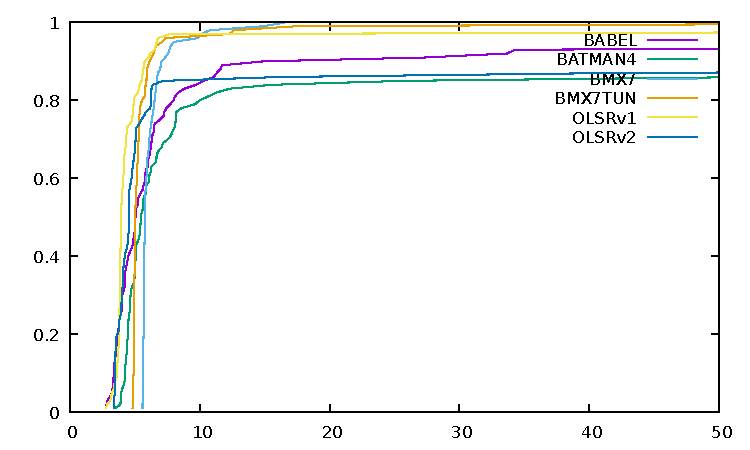
\includegraphics[width=0.48\linewidth]{images/cdf-failuretest-node8-fc00:2::1.pdf}

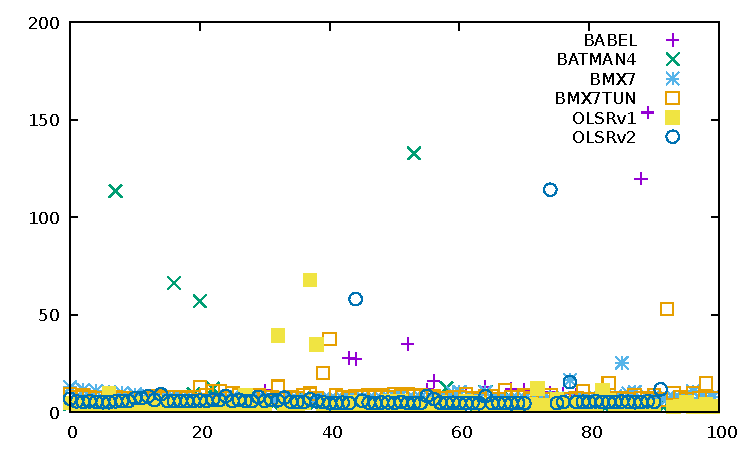
\includegraphics[width=0.48\linewidth]{images/scatter-failuretest-node9-fc00:2::1.pdf}\hfill%
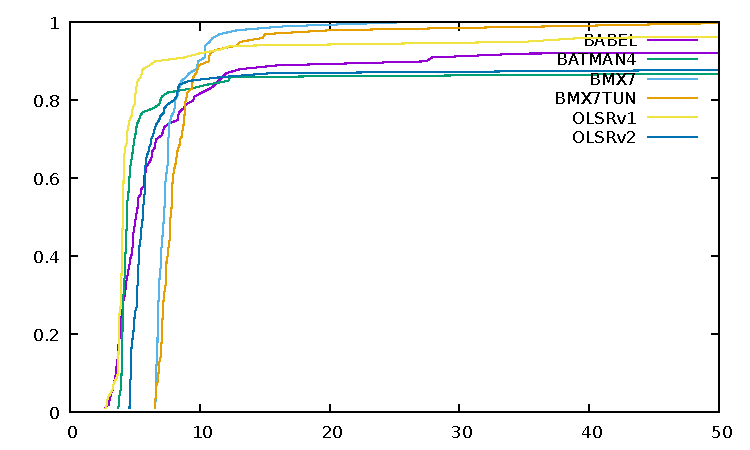
\includegraphics[width=0.48\linewidth]{images/cdf-failuretest-node9-fc00:2::1.pdf}
\caption{Time-sequence and CDF plots of the ping data (links 8-17, 8-2, 9-17, 9-2).}\label{fig:jch}
\end{figure}

CDF diagrams for the same data (omitting BATMAN5, which adds too much
noise to the figures) are presented in Figure~\ref{fig:jch}.

\FloatBarrier
\subsection{iperf Test}
\Cref{fig:iperfnoflows,fig:iperfoneflow,fig:iperffourflows} report the performance
of all the protocols when two parallel iperf sessions are run to measure the
performance and zero, one or 4 sessions are added to increase background noise.
The background sessions are fixed at 5Mbps and take place between couples
(14,10), (4,15), (1,16), (12,11). Some observations that can be done are:
\bi
\ii There is a net performance degradation from one figure to the next one. 
\ii With zero and one flow, in the path 8-17 (that according to \cref{fig:ETXrank}
is the shortest of the two) the protocol behave similarly, while in the path 9-2
there is a higher performance variation. In particular, BMX7 consistently
performs better than the others (as the median value) but also shows the largest
deviation. This may be the consequence of the combination of the zero loss and
the stable delay that BMX7 is able to obtain (see \cref{fig:pingloss,fig:delaydist}).
\ii with 5 flows, the relative difference increases and OLSRv2 seems to perform
better than the other protocols averaging the results of both paths.
\ei


\begin{figure}[!htb]
  \centering
    \includegraphics[width=.9\linewidth]{images/failure_test_iperf_10runs-IPv6.png}
    \caption{iperf tests without background traffic.}
  \label{fig:iperfnoflows}
\end{figure}

\begin{figure}[!htb]
  \centering
    \includegraphics[width=.9\linewidth]{images/failure_test_iperf_10runs-IPv6-oneflow.png}
    \caption{iperf tests with one background traffic flow.}
  \label{fig:iperfoneflow}
\end{figure}

\begin{figure}[!htb]
  \centering
    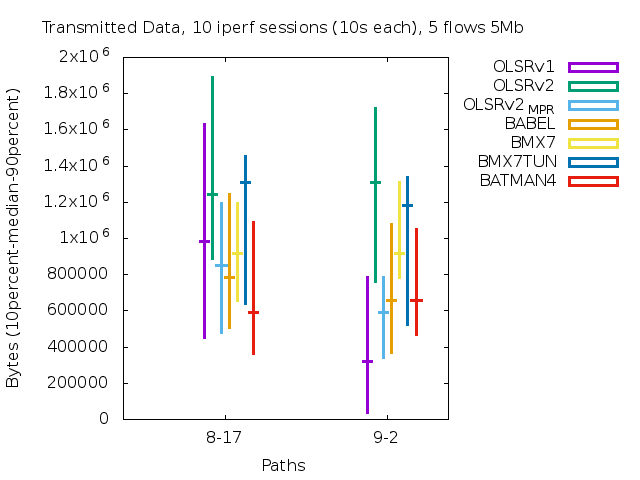
\includegraphics[width=.9\linewidth]{images/failure_test_iperf_10runs-IPv6-twoflow.png}
    \caption{iperf tests with four background traffic flows.}
  \label{fig:iperffourflows}
\end{figure}

\Cref{fig:iperfnofair} reports the comparison of the performance of the iperf
sessions, without background traffic with and without the Airtime fairness
enabled. Each color in the figure corresponds to a protocol, the left value
(with a dot at the median value) is the performance without the Airtime fairness
enabled, the right value (with a dash at the median value) is the performance
with the Airtime fairness enabled. It is hard to draw any conclusion on the
importance of Airtime fairness, BMX7 still remains the protocol that guarantees
the highest throughput, even if it is affected by the Airtime fairness in the
opposite way in the two paths. Also the other protocols are affected both positively
and negatively by Fairness, so it is unclear if the results are the effect of
fairness, or of the changed conditions in the testbed from one run to the other.
The only conclusion is that Airtime fairness does not influence the performance
of mesh protocols in an critical way. 


\begin{figure}[!htb]
  \centering
    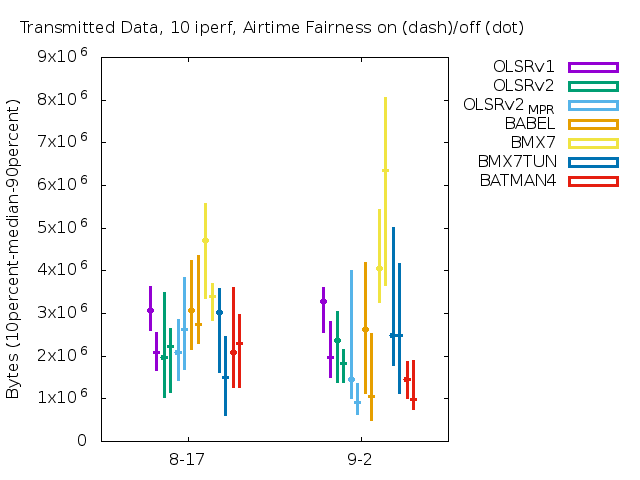
\includegraphics[width=.9\linewidth]{images/failure_test_iperf_10runs-IPv6_noairfair.png}
    \caption{iperf tests without background traffic and with/without airtime fairness.}
  \label{fig:iperfnofair}
\end{figure}

\FloatBarrier
\section{Suggestion for the Future Battlemeshers}

What follows is a set of recommendations we, as the people that spent most time
on the testbed, want to give to the ones that in the next editions of the
battlemesh will set-up the testbed. 


\begin{mybox}{Assign micro-tasks to other people}
    Setting up the testbed is full-time activity, so it is demanding on those
    that do it. Still, some tasks can be ``outsourced'' to others, tasks that
    are small, atomic and tedious, such as writing scripts to parse the output
    of commands  used for testing (ping, iperf, traceroute\ldots). When needed,
    instead of spending tens of minutes to write the script, it is useful to ask
    for help to others, this was done a couple of times and worked good.
    Ideally: write the task to an etherpad, ring a bell, and wait for someone to
    provide a script that does the job.
\end{mybox}

\begin{mybox}{Use cables!}
    We choose 802.11s for the management network because, if it does not work,
    we can't blame any of the protocols under test. 802.11s works decently but,
    as any other solution is influenced by the state of the network. We believe
    that the best thing would be to buy a 300M reel of ethernet cable, and use
    that to manage the nodes. This would spare us of many failures in
    connecting, launching scripts, failing, restarting etc\ldots. Powerline
    could be an alternative.
\end{mybox}
\begin{mybox}{Do small tests}
    Large scale tests (all nodes against all nodes) are tempting, but since the
    network becomes complex it is hard to understand what is happening. We
    decided to start with small tests, where it is easier to understand what
    happens, while it happens. 
\end{mybox}
\begin{mybox}{Bring hardware for night-time tests}
    Probably the best moment to perform large-scale tests is during the night.
    But no one wants to leave his/her laptop at the BM nighttime. So it is
    important to remember to bring some other hardware (like a few raspberries)
    that can be used to perform automated tests during the night. 
\end{mybox}

\begin{mybox}{Fork the testbed}
    It happens that some of the devels need to use the testbed to fix bugs that
    happen during the experiments, and it is the added value of BM for them. On
    the other side, we can not freeze testing for long while they debug/improve
    their code. So a wise idea is to realize a small tbed (4-5 nodes) detached
    from the large one that devels can use to fix their bugs. 
\end{mybox}


\section{Conclusions}
While there is a discussion in the BM community about changing the format of the event
to something that is more conference-wise and less testbed-wise, our
impression is that the testbed is important. Even if the results are
incomplete, and scientifically not always sound, the whole process of
setting up the testbed, running the protocols, debugging with the developers
is an integral part of the conference and guarantees that the experts will
participate to the conference, which makes it different from any other
conference. 



%\bibliographystyle{IEEEtran}
%\bibliography{bibliography}


\end{document}


